\documentclass[../main.tex]{subfiles}
\begin{document}
\subsection{Coordinate polari}
\begin{itemize}
    \item Coordinate cartesiane, $P=(x,y)$ (ascissa, ordinata)
    \item Coordinate polari, $P=(r,\alpha)$ (norma, angolo)
\end{itemize}
\vspace{1cm}

Per passare da coordinate polari a coordinate cartesiane si utilizzano rispettivamente $cos(\alpha)$ e $sin(\alpha)$. Vale dunque:
$$
    \begin{cases}
        x = r\phantom{.}cos(\alpha) \\
        y = r\phantom{.}sin(\alpha)
    \end{cases}
$$
che graficamente appare:
\begin{figure}[h]
    \centering
    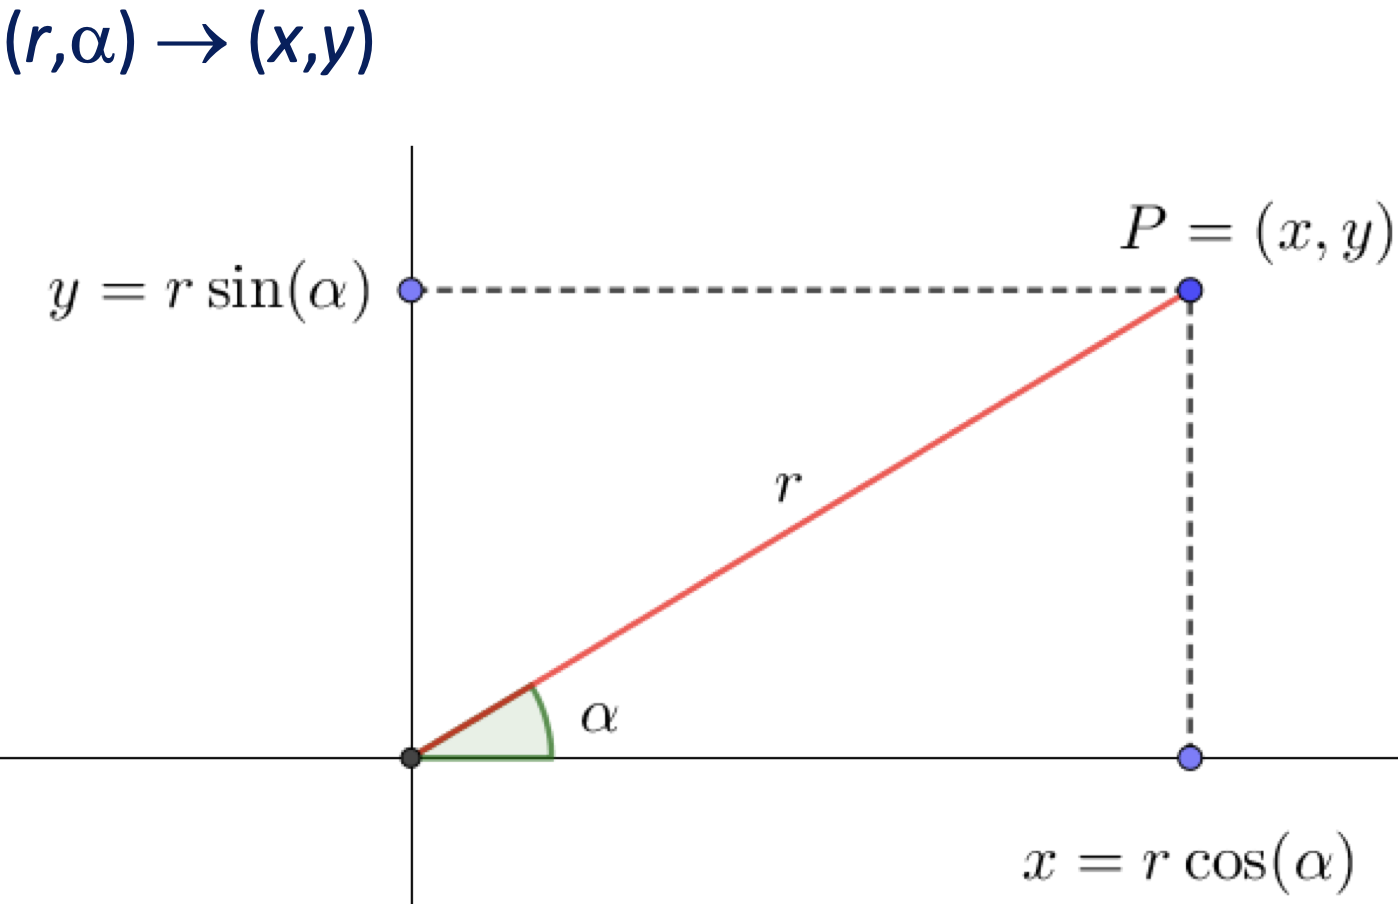
\includegraphics[width=0.6\textwidth]{../images/polariCartesiane.png}
\end{figure}

\vspace{2cm}
Per passare invece da coordinate cartesiane a coordinate polari dobbiamo stabilire $r$ e $\alpha$. Abbiiamo quindi:
$$
    \begin{cases}
        r = \sqrt{x^2 + y^2} \\
        \alpha = \begin{cases}
            cos^{-1}(\frac{x}{r}) \phantom{--} y \geq 0 \\
            -cos^{-1}(\frac{x}{r}) \phantom{-} y < 0
        \end{cases}
    \end{cases}
$$
che graficamente appare:
\begin{figure}[h]
    \centering
    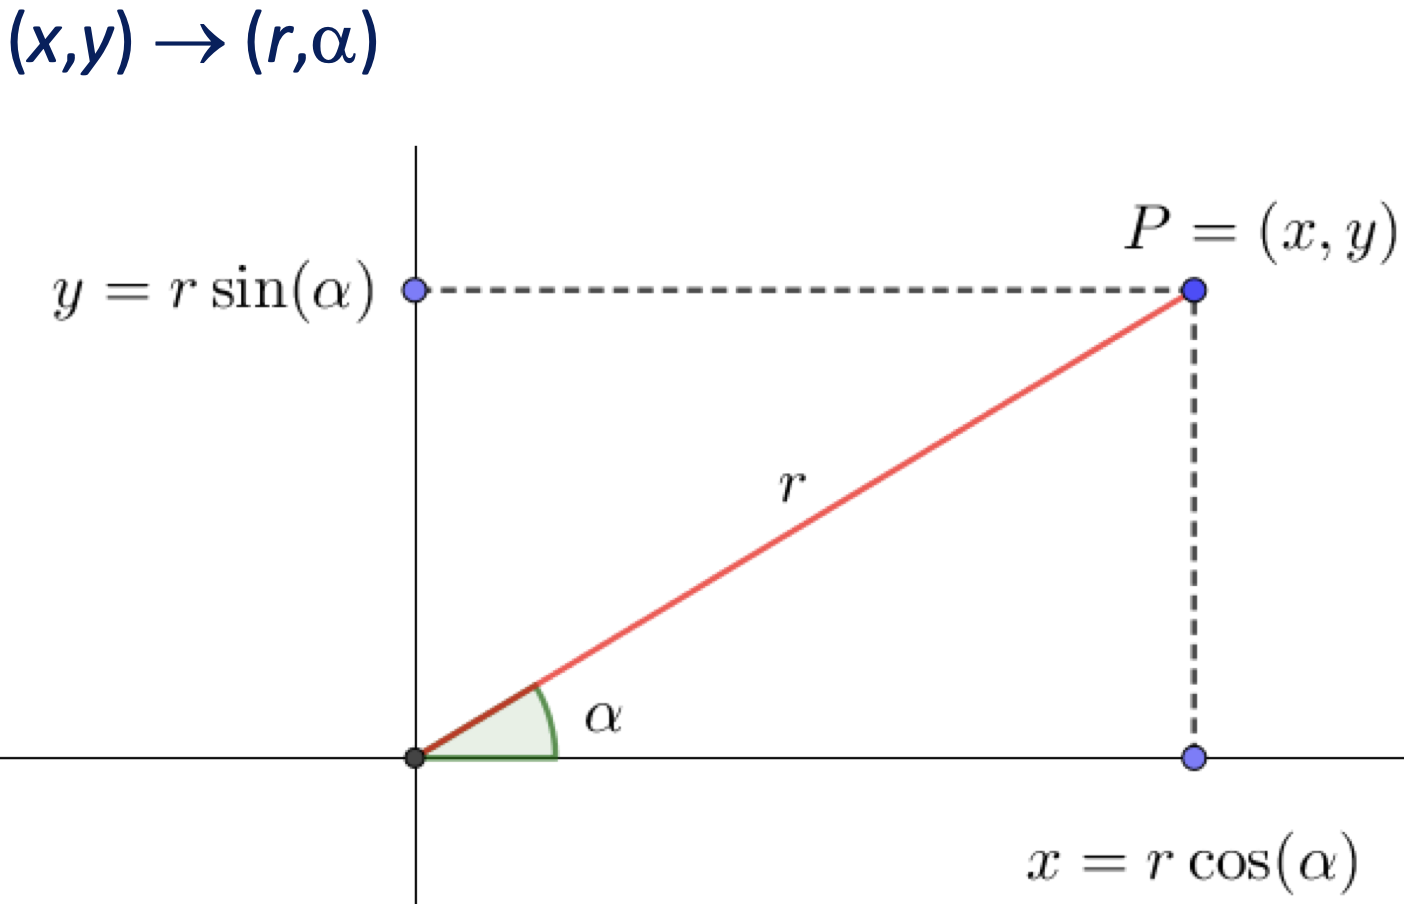
\includegraphics[width=0.6\textwidth]{../images/cartesianePolari.png}
\end{figure}

\subsection{Il prodotto scalare}
\subsubsection{norma}
Dato il vettore $x$ si chiama prodotto scalare di $x$ per se stesso e si indica $x \cdot x$ il numero reale
$$
   \mathbb{R}^2 \text{: } x \cdot x = \begin{pmatrix} x_1 \\ x_2 \end{pmatrix} \cdot \begin{pmatrix} x_1 \\ x_2 \end{pmatrix} 
   = x^2_1 + x^2_2 = \left\lVert x \right\rVert^2
$$
dunque la norma è
$$
    \left\lVert x \right\rVert = \sqrt{x \cdot x}
$$
questo vale in qualsiasi dimensione ($\mathbb{R}^n$).

\vspace{0.5cm}
La norma è un valore sempre maggiore o, nel caso il vettore fosse nullo, uguale a zero. Inoltre possiede due proprietà interessanti:
\begin{itemize}
    \item \textbf{disuguaglianza triangolare}, $\left\lVert x + y \right\rVert \leq \left\lVert x \right\rVert + \left\lVert x \right\rVert$
    \item \textbf{omogeneità}, $\left\lVert hx \right\rVert = \left\lvert h \right\rvert + \left\lVert x \right\rVert $
\end{itemize}
La somma di due norme non è quindi uguale alla norma contenente la somma dei due vettori (disuguaglianza triangolare).

\subsubsection{I versori}
I versori sono vettori di norma $1$, per fare diventare un vettore generico $\left\lVert x \right\rVert$ di norma $1$ si può fare
$$
    \frac{1}{\left\lVert x \right\rVert } x  \phantom{--}\text{ questo vettore ha norma 1}
$$

Allo stesso modo se vogliamo farlo diventare, per esempio, di norma $7$ possiamo scriverlo come
$$
    \frac{7}{\left\lVert x \right\rVert } x \phantom{--} \text{ questo vettore ha norma 7}
$$

\subsubsection{Prodotto scalare x$\cdot$y}
Dati i vettori $x = \begin{pmatrix}x_1 \\ x_2 \\ ... \\ x_n \end{pmatrix}, y = \begin{pmatrix}y_1 \\ y_2 \\ ... \\ y_n \end{pmatrix} \in \mathbb{R}^n$,
si chiama prodotto scalare di $x$ e $y$, e si indica $x \cdot y$, il numero reale
$$
    x \cdot y = x_1y_1 + x_2y_2 + ... + x_ny_n
$$

Di base se prendiamo due vettori tramite l'agolo che generano possiamo determinare:
\begin{itemize}
    \item se $\alpha > 90^{\circ}$ il prodotto scalare è negativo
    \item se $\alpha = 90^{\circ}$ il prodotto scalare è $0$
    \item se $\alpha < 90^{\circ}$ il prodotto scalare è positivo
\end{itemize}

\vspace{1cm}
\textbf{Teorema del prodotto scalare}
$$
   u \cdot v = \left\lVert u \right\rVert \left\lVert v \right\rVert cos(\alpha)
$$
dalla quale possiamo ricavare
$$
    cos(\alpha) = \frac{u \cdot v}{\left\lVert u\right\rVert \left\lVert v\right\rVert }
$$
e quindi
$$
    \alpha = cos^{-1}\left( \frac{u \cdot v}{\left\lVert u \right\rVert \left\lVert v \right\rVert } \right)
$$
\textbf{Nota:} $\alpha rad = \frac{\pi}{180} \alpha^\circ $
\end{document}